\documentclass[border=10pt]{standalone}
\usepackage[svgnames]{xcolor}
\usepackage{amsmath}
\usepackage{pgfplots}
\pgfplotsset{compat=newest}
\usepackage[sfdefault]{FiraSans}
\usepackage{FiraMono}
\renewcommand*\familydefault{\sfdefault}
\begin{document}
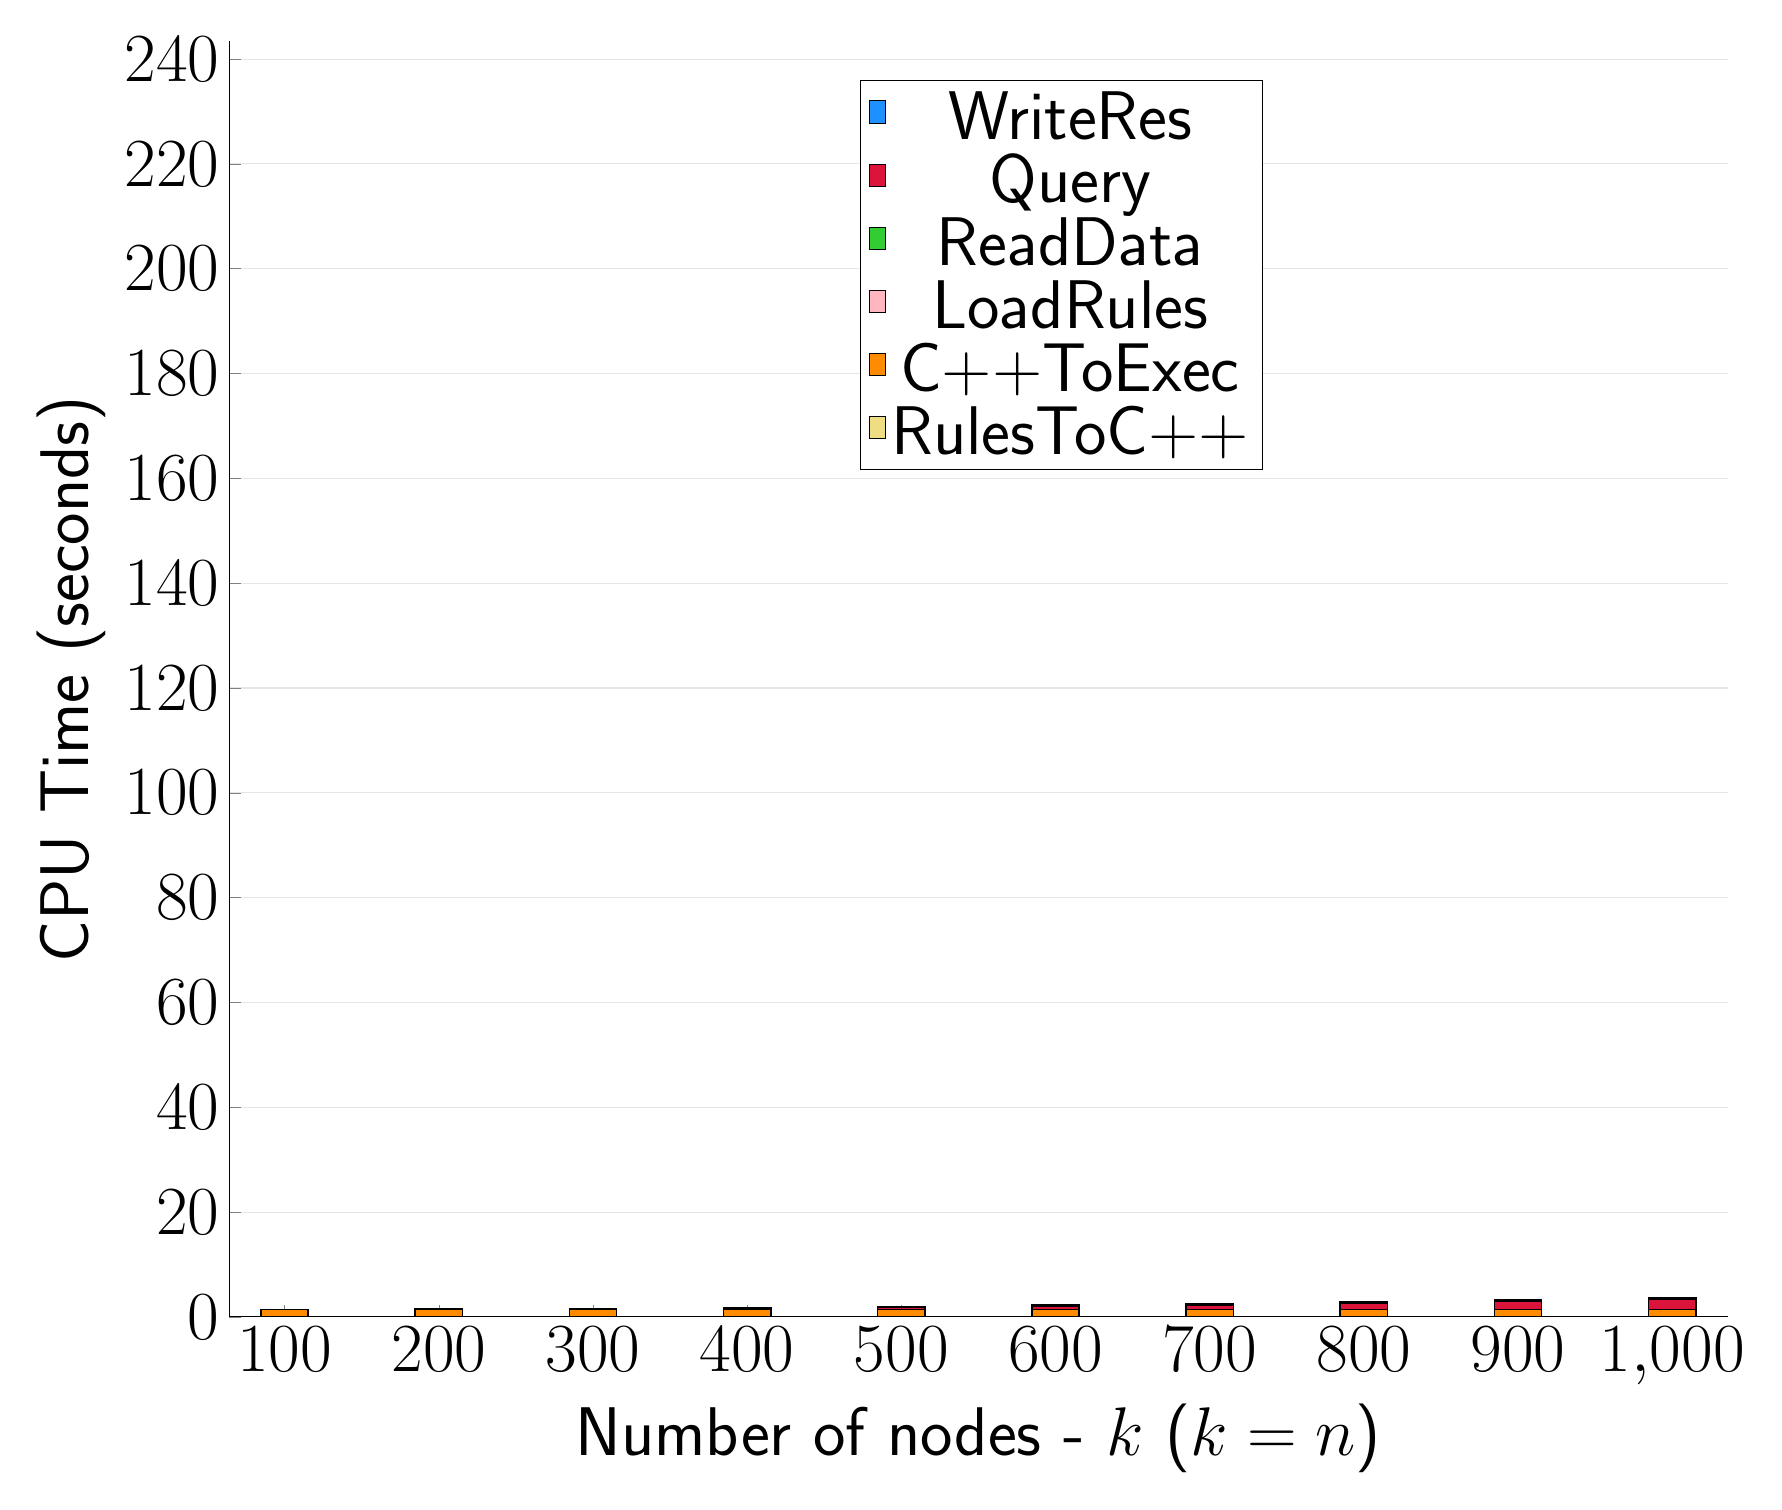
\begin{tikzpicture}
\begin{axis}[
   ybar stacked,
   width=1.7\textwidth,
   bar width=0.6cm,
   ymajorgrids, tick align=inside,
   major grid style={draw=gray!20},
   xtick=data,
   ymin=0, ymax=243.3584,
   axis x line*=bottom,
   axis y line*=left,
   enlarge x limits=0.04,
   legend style={
       at={(0.69, 0.97)},
       anchor=north east,
       legend columns=1,
       font=\Huge,
   },
   ylabel={CPU Time (seconds)},
   xlabel={Number of nodes - $k$ ($k=n$)},
   label style={font=\Huge},
   tick label style={font=\Huge},
]
\addlegendimage{fill=DodgerBlue, draw=black, line width=0.2pt}
\addlegendentry{WriteRes}
\addlegendimage{fill=Crimson, draw=black, line width=0.2pt}
\addlegendentry{Query}
\addlegendimage{fill=LimeGreen, draw=black, line width=0.2pt}
\addlegendentry{ReadData}
\addlegendimage{fill=LightPink, draw=black, line width=0.2pt}
\addlegendentry{LoadRules}
\addlegendimage{fill=DarkOrange, draw=black, line width=0.2pt}
\addlegendentry{C++ToExec}
\addlegendimage{fill=LightGoldenrod, draw=black, line width=0.2pt}
\addlegendentry{RulesToC++}
\addplot +[fill=LightGoldenrod, draw=black, line width=0.55pt] coordinates {
(100, 0.006)
(200, 0.006000000000000003)
(300, 0.006000000000000005)
(400, 0.003999999999999998)
(500, 0.007999999999999997)
(600, 0.009999999999999998)
(700, 0.003999999999999998)
(800, 0.003999999999999998)
(900, 0.006)
(1000, 0.005999999999999997)
};
\addplot +[fill=DarkOrange, draw=black, line width=0.55pt] coordinates {
(100, 1.3940000000000001)
(200, 1.4620000000000002)
(300, 1.4360000000000002)
(400, 1.3800000000000001)
(500, 1.392)
(600, 1.4140000000000001)
(700, 1.3960000000000004)
(800, 1.4000000000000004)
(900, 1.372)
(1000, 1.372)
};
\addplot +[fill=LightPink, draw=black, line width=0.55pt] coordinates {
(100, 0.000113)
(200, 0.000156)
(300, 0.0001644)
(400, 0.0001536)
(500, 0.0001406)
(600, 0.0001434)
(700, 0.000115)
(800, 0.0001082)
(900, 0.00014819999999999997)
(1000, 0.00014099999999999998)
};
\addplot +[fill=LimeGreen, draw=black, line width=0.55pt] coordinates {
(100, 0.0007693999999999999)
(200, 0.0015172000000000002)
(300, 0.0016534)
(400, 0.0023740000000000002)
(500, 0.0030864000000000004)
(600, 0.0035223999999999997)
(700, 0.0035202000000000002)
(800, 0.0041605999999999995)
(900, 0.005353200000000001)
(1000, 0.0051354)
};
\addplot +[fill=Crimson, draw=black, line width=0.55pt] coordinates {
(100, 0.0240936)
(200, 0.08407300000000001)
(300, 0.1700792)
(400, 0.2912916)
(500, 0.45283860000000004)
(600, 0.6859024)
(700, 0.9016770000000001)
(800, 1.194874)
(900, 1.5825939999999998)
(1000, 1.889606)
};
\addplot +[fill=DodgerBlue, draw=black, line width=0.55pt] coordinates {
(100, 0.0044608)
(200, 0.012864800000000001)
(300, 0.028742800000000002)
(400, 0.0509436)
(500, 0.077478)
(600, 0.11246099999999999)
(700, 0.1545972)
(800, 0.1997032)
(900, 0.2561948)
(1000, 0.31440619999999997)
};
\end{axis}
\end{tikzpicture}

\end{document}
